線形回帰とは与えられたデータに対し, 線形関数を当てはめる問題である.
\begin{center}
    \begin{tikzpicture}[>=stealth]
        \draw[->] (-4,0)--(4,0) node[right] {$x$};
        \draw[->] (0,-0.5) --(0,4) node[above] {$y$};
        \node at(-0.2,-0.2) {O};
        \draw[thick,domain=-3.5:4] plot(\x,{\x/2+1});
        \draw[fill=white] (0,0.9) circle[radius=0.05];
        \draw[fill=white] (-0.5,0.95) circle[radius=0.05];
        \draw[fill=white] (0.5,1.5) circle[radius=0.05];
        \draw[fill=white] (1,1) circle[radius=0.05];
        \draw[fill=white] (1.5,1.9) circle[radius=0.05];
        \draw[fill=white] (2,1.7) circle[radius=0.05];
        \draw[fill=white] (3,2.6) circle[radius=0.05];
        \draw[fill=white] (-2.2,0) circle[radius=0.05];
        \filldraw (1,1.5) circle[radius=0.05];
        \draw[<->,draw=blue,thick] (1,1.45)--(1,1.05);
        \node at(0.8,1.9) {$(x_{i},\tilde{y}_{i})$};
        \node at(1,0.7) {$(x_{i},y_{i})$};
        \node at(1.3,1.1) {$e_{i}$};
    \end{tikzpicture}
\end{center}
すると推測される関数は以下のように表すことができる.
\begin{eqnarray*}
    \tilde{y}_{i}=f(x_{i};a,b) = ax_{i}+b
\end{eqnarray*}
このとき, 誤差$e_{i}$は
\begin{eqnarray*}
    e_{i}=|\tilde{y}_{i}-y_{i}|
\end{eqnarray*}
となるので, これの二乗したときの最小を求めれば最適化される. つまり
\begin{align*}
    \underset{a,b}{\rm min} \sum_{i=1}^{N}e_{i}^{2} = \underset{a,b}{\rm min} \sum_{i=1}^{N}\left(\tilde{y}_{i}-y_{i}\right)^{2} \tag{2.1}
\end{align*}
を求めればよい. これを求める方法を最小二乗法である.\\
$(x_{n},y_{n})$\ :\ $n$番目の学習データ\\
$\mbox{\boldmath $x$}_{n}=\begin{bmatrix}x_{n}&1\end{bmatrix}^{T}$\ :\ $x_{n}$を次元拡張したベクトル\\
$D = \begin{bmatrix}\mbox{\boldmath $x$}_{1}&\mbox{\boldmath $x$}_{2}&\cdots&\mbox{\boldmath $x$}_{n} &\cdots \end{bmatrix}^{T}\ =\ \begin{bmatrix}d_{ij}\end{bmatrix},\ \ (d_{i1}=x,\ d_{i2}=1)$\\
$\mbox{\boldmath $w$}^{T} = \begin{bmatrix} a&b \end{bmatrix}$\\
$\tilde{y}_{n} = ax_{n}+b = \begin{bmatrix} a&b \end{bmatrix} \begin{bmatrix} x_{n}\\1 \end{bmatrix}=\mbox{\boldmath $w$}^{T}\mbox{\boldmath $x$}_{n} = \displaystyle \sum_{k=1}^{2}w_{k}\cdot d_{nk}$\\
$\mbox{\boldmath $\tilde{y}$} = D\mbox{\boldmath $w$}$\\
$\mbox{\boldmath $e$}=\begin{bmatrix}e_{1}\\e_{2}\\\vdots \\ e_{n}\\ \vdots \end{bmatrix}=\begin{bmatrix}e_{n}\end{bmatrix},\ \ e_{n}=\tilde{y}_{n}-y$\\
ここで誤差$E$は二乗誤差の$\displaystyle \frac{1}{2}$倍したものと定義し,
\begin{eqnarray*}
    E&=&\frac{1}{2}\mbox{\boldmath $e$}^{T} \mbox{\boldmath $e$} = \frac{1}{2}\left(\mbox{\boldmath $\tilde{y}$} -\mbox{\boldmath $y$} \right)^{T}\left(\mbox{\boldmath $\tilde{y}$} -\mbox{\boldmath $y$} \right)\\
    &=&\frac{1}{2}\left(D\mbox{\boldmath $w$}-\mbox{\boldmath $y$}\right)^{T}\left(D\mbox{\boldmath $w$}-\mbox{\boldmath $y$}\right)
\end{eqnarray*}
ここで誤差が最小となるときは$\displaystyle \frac{\partial E}{\partial \mbox{\boldmath $w$}}=0$となるときである.\\
ここで
\begin{eqnarray*}
    &&\frac{\partial}{\partial \mbox{\boldmath $x$}} \mbox{\boldmath $x$}^{T}\mbox{\boldmath $a$} = \mbox{\boldmath $a$}\\
    &&\frac{\partial}{\partial \mbox{\boldmath $x$}} \mbox{\boldmath $a$}\mbox{\boldmath $x$} = \mbox{\boldmath $a$}^{T}\\
    &&\frac{\partial}{\partial \mbox{\boldmath $x$}}\mbox{\boldmath $x$}^{T}\mbox{\boldmath $x$}=2\mbox{\boldmath $x$}
\end{eqnarray*}
という性質を使えば微分をすることができて, 微分する項を展開して微分すると以下のようになる.
\begin{eqnarray*}
\frac{\partial E}{\partial \mbox{\boldmath $w$}}&=&\left(\frac{1}{2}(D\mbox{\boldmath $w$}-\mbox{\boldmath $y$})^{T}(D\mbox{\boldmath $w$}-\mbox{\boldmath $y$})\right)'\\
                                                &=& \frac{1}{2}\left(\mbox{\boldmath $w$}^{T}D^{T}D\mbox{\boldmath $w$}-\mbox{\boldmath $w$}^{T}D^{T}\mbox{\boldmath $y$}-\mbox{\boldmath $y$}^{T}D\mbox{\boldmath $w$}+\mbox{\boldmath $y$}^{T}\mbox{\boldmath $y$}\right)'\\
                                                &=& \frac{1}{2}\left(D^{T}D\mbox{\boldmath $w$}+(\mbox{\boldmath $w$}^{T}D^{T}D)^{T}-D^{T}\mbox{\boldmath $y$}-(\mbox{\boldmath $y$}^{T}D)^{T}\right)\\
                                                &=& \frac{1}{2}(D^{T}D\mbox{\boldmath $w$}+D^{T}D\mbox{\boldmath $w$}^{T}-D^{T}\mbox{\boldmath $y$}-D^{T}\mbox{\boldmath $y$})\\
&=& D^{T}D\mbox{\boldmath $w$}-D^{T}\mbox{\boldmath $y$}
\end{eqnarray*}
であるから,
\begin{eqnarray*}
    &&\frac{\partial E}{\partial \mbox{\boldmath $w$}} = D^{T}D\mbox{\boldmath $w$}-D^{T}\mbox{\boldmath $y$}=0\\
    \Longleftrightarrow&&\  D^{T}D\mbox{\boldmath $w$} = D^{T}\mbox{\boldmath $y$}\\
    \Longleftrightarrow&&\  \mbox{\boldmath $w$} = \left(D^{T}D\right)^{-1}D^{T}\mbox{\boldmath $y$}
\end{eqnarray*}
となる.
$(-2,0),\ (-1,-1),\ (0,1),\ (1,3),\ (2,2)$のとき, 最小二乗法を用いて線形回帰モデルを求める.
\begin{center}
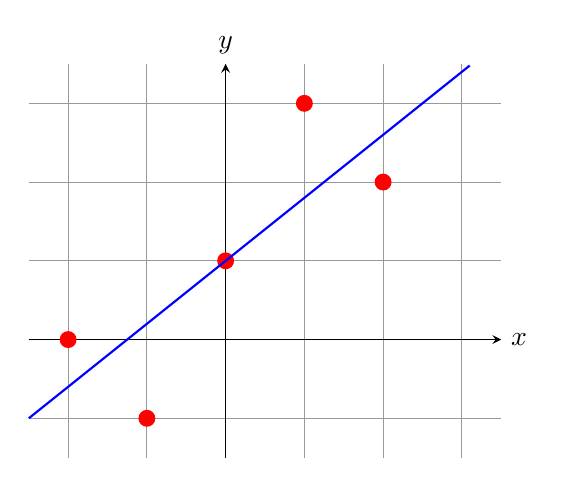
\begin{tikzpicture}[>=stealth]
    \draw[draw=gray!80] (-2.5,-1.5) grid (3.5,3.5);
    \draw[->](-2.5,0)--(3.5,0) node[right] {$x$};
    \draw[->](0,-1.5)--(0,3.5) node[above] {$y$};
    \filldraw[fill=red,draw=red] (-2,0) circle[radius=0.1];
    \filldraw[fill=red,draw=red] (-1,-1) circle[radius=0.1];
    \filldraw[fill=red,draw=red] (0,1) circle[radius=0.1];
    \filldraw[fill=red,draw=red] (1,3) circle[radius=0.1];
    \filldraw[fill=red,draw=red] (2,2) circle[radius=0.1];
    \draw[domain=-2.5:3.1,thick,draw=blue] plot(\x,{\x*0.8+1});
\end{tikzpicture}
\end{center}
pythonでの実装方法は以下である.
\lstinputlisting{np.py}

説明変数が多変数の場合も同様にして考えることができ, 以下のようになる.\\
$(x_{n1},x_{n2},\cdots,x_{np},y_{n})$\ :\ $n$番目の学習データ\\
$\mbox{\boldmath $x$}_{n} = \begin{bmatrix}x_{n1}&x_{n2}&\cdots &x_{np}&1\end{bmatrix}^{T}$\\
$D=\begin{bmatrix}\mbox{\boldmath $x$}_{1}&\mbox{\boldmath $x$}_{2}&\cdots &\mbox{\boldmath $x$}_{i}&\cdots&\mbox{\boldmath $x$}_{N}\end{bmatrix}^{T}$\ :\ データ行列\\
$\mbox{\boldmath $w$}=\begin{bmatrix}a_{1}&a_{2}&\cdots &a_{p}&b \end{bmatrix}^{T}$\ :\ パラメタ\\
    $\mbox{\boldmath $y$} = D\mbox{\boldmath $w$}$\ :\ 予測式\\
    $\mbox{\boldmath $w$}=(D^{T}D)^{-1}D^{T}\mbox{\boldmath $y$}$\\[1cm]
    以下の12点から線形回帰モデルを最小二乗基準で求める.\\
(0,0,1),\ (0,1,3),\ (0,2,2),\ (0,3,3),\ (1,0,1),\ (1,1,4),\ (1,2,5),\ (1,3,4),\ (2,0,4),\ (2,1,5),\ (2,2,4),\ (2,3,7)\\[1cm]
pythonでの実行すると
\begin{eqnarray*}
    \mbox{\boldmath $\tilde{y}$} = 1.375x_{1}+0.76666667x_{2}+1.05833333
\end{eqnarray*}
となる.\\
一方で次の9点から, 線形回帰モデルを最小二乗基準で求める.\\
(0,0,1),\ (1,2,3),\ (2,4,2),\ (3,6,2),\ (4,8,3),\ (5,10,1),\ (6,12,4),\ (7,14,5),\ (8,16,4)\\[1cm]
これは逆行列が存在しないので, 最小二乗法での解は存在しない.\\
